\section*{Chapitre 2}
\section{Spécification}
\subsection{Faisabilité du projet}
Dans un premier temps, nous avons suivi un cours sur \url{www.udacity.com} pour apprendre la base des connaissances de développer une application sous Android. Ce cours nous a permis de développer nous-même une simple application, par exemple un compteur de points qui est utilisé dans un match du basket, sous Android. 

\indent Ensuite, nous avons effectué une brève étude bibliographique quant à la faisabilité du développent des fonctionnalités que nous avons proposées. Nous avons trouvé des APIs du développement sous Android. Dans ce cas là, nous pensions que tous les fonctionnalités pouvaient être développées sous Android sans trop de difficultés.

\indent Concernant la partie de la réponse intelligente, comme les anciens PAOs ont travaillé sur ce sujet, nous avons décidé d'utiliser le Pandorabots, outil Internet permettant d'héberger un grand nombre de fichiers AIML contenant les questions/réponses, pour nous aider de réaliser toutes les fonctionnalités. Le choix de l'IDE a été fait rapidement, nous avons choisi Android Studio qui est un IDE très moderne.

\indent Notre application peut fonctionner sur Android 4.4 ou supérieur avec une connexion Internet permanante.\\

\subsection{Analyse Descendante}
\begin{figure}[h]
\centering
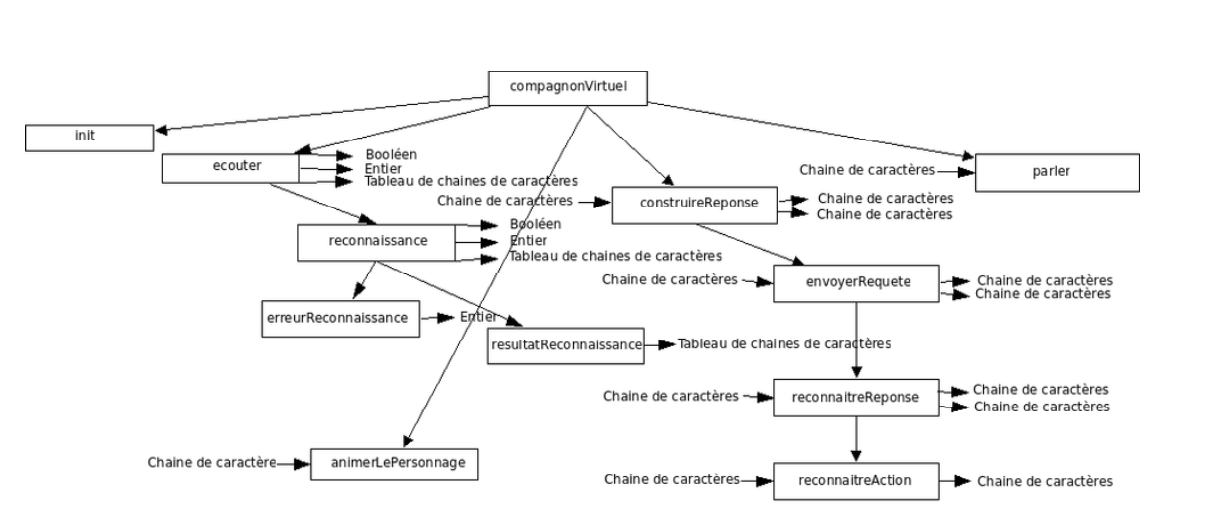
\includegraphics[width=1\linewidth]{analyseDescendante.png}
\caption{Analyse descendante de la version ancienne.\label{fig1}}
\end{figure}
\indent L'analyse descendante a été décrite dans le rapport de 1ère version.
\newpage
